\clearpage
\section{Einleitung}
\label{sec:Einleitung}

Eine gelungene Party auf die Beine zu stellen verlangt einem einiges ab. Vor allem kostet es eine Menge Aufwand und Zeit. Dies gilt besonders, wenn es darum geht mit vielen Freunden zusammen zu feiern. Neben der gelungenen Musikauswahl und den Snacks dürfen die Getränke auf keinen Fall fehlen. Um diese sicherzustellen, gibt es mehrere Möglichkeiten. Einerseits könnte jeder seine eigenen Getränke mitbringen, was jedoch bedeutet, dass es unter Umständen eine riesige Sauerei gibt oder viele Flaschen in der Gegend rumstehen. Anderseits könnte man als Gastgeber selber anbieten Cocktails zu mixen und so den Getränkenachschub zu gewährleisten. Da gibt es jedoch ein grosses Problem. Als Gastgeber möchte man nicht den ganzen Abend hinter der Bar stehen müssen, sondern lieber bedenkenlos mitfeiern.

Damit genau dies möglich ist, wurde der PartyMixer geschaffen. Dieses System soll dem Anwender eine einfache Cocktailerstellung dank dem innovativen Zusammenspiel von intuitiven Komponenten bieten. Ein Mikrocontroller bildet dabei das Herz dieser Cocktailmaschine, welche mit der aus C-Code bestehenden Software alle Komponenten wie Pumpen, Durchflussmessgeräte und Motor ansteuert. Unterstützt wird dieser von einem Wireless- / Bluetoothmodul, welches für zusätzliche Schnittstellen sorgt und eine Anbindung einer App oder eines Webhostes ermöglicht. Weitere Systeme wie RFID oder Beleuchtungssysteme runden das Paket als gesamtes ab. 

Ein stabiles Rahmensystem bildet das Grundgerüst einer voll umfänglich entwickelten Mechanik, welche nicht nur Die Elektronik und deren Komponenten beinhaltet, sondern auch die Flüssigkeiten. Eine Kältekammer sorgt hierbei für ideale Getränketemperaturen. 

All diese Komponenten interagieren gemäss Blockbild in Abbildung \ref{fig:Konzept_Partymixer} zusammen.


\begin{figure}[h!]
\center
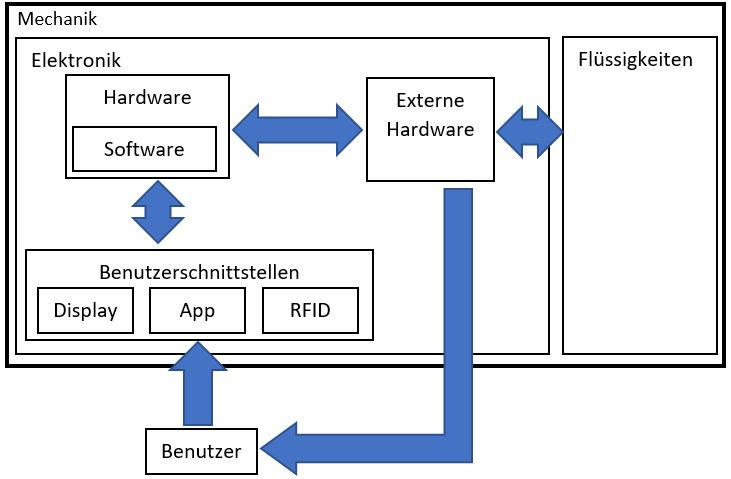
\includegraphics[width = 0.6\textwidth]{graphics/Konzept}
\caption{Konzept des PartyMixer's}
\label{fig:Konzept_Partymixer}
\end{figure}

In den folgenden Kapiteln ist dokumentiert, wie die Cocktailmaschine im Detail aussieht und wie die einzelnen Teilsysteme aufgebaut sind. Dazu gehören die elektronischen Teilsysteme, das dazugehörige Printdesign, die Software und die Mechanik. In Kapitel \ref{sec:Mechanik} wird die komplette Mechanik beschrieben, wohingegen in Kapitel \ref{sec:Printaufbau} und \ref{sec:Teilsysteme} die Elektronik unter die Lupe genommen wird. Ausserdem wird in \ref{sec:Inbetriebnahme} das  System in Betrieb genommen.  